
% LaTeX template for extended abstract submissions to the 2nd International Conference on
% Models and Technologies for Intelligent Transportation Systems
% 22-24 June, 2011, Leuven, Belgium
% Please do not change the layout of the document. Example text that should be substituted for
% abstract submission is marked by "EDIT" with a description of what to fill in.

% WARNING: Skip to title. Do not change these definitions
\documentclass[a4paper,10pt,twocolumn]{article}

\usepackage[a4paper,top=3cm,bottom=2.7cm,left=2cm,right=2cm]{geometry}	% Page formatting
\usepackage[english]{babel}																							% Hyphenations
\usepackage{amsthm}																											% Maths
%\usepackage{graphicx,subfigure}																					% Figures
\usepackage{graphicx}
%\usepackage{lscape}																											% Indentation
\usepackage{fancyhdr}																										% Document header
\usepackage[calcwidth]{titlesec}																										% Sections and subsections layout
\usepackage[hang,small,bf]{caption}
\usepackage{hyperref}
\usepackage{makeidx}
\usepackage{subcaption}
\usepackage[]{algorithm2e}
\usepackage{longtable}
\usepackage{listings}
\usepackage{color}
\usepackage{rotating}
\usepackage{float}
\usepackage{placeins}
%appendix
\usepackage[title,titletoc,toc]{appendix}
\usepackage{dblfloatfix} 


\renewcommand{\headrulewidth}{0pt}
\setlength{\headheight}{35pt}
\pagestyle{fancyplain}
\fancyhf{}
\chead{\fancyplain{}{First draft of the scientific paper for the thesis Visualization of music suggestions by Joris Schelfaut}}
\addto\captionsenglish{
				\renewcommand{\abstractname}{ABSTRACT}
				\renewcommand{\refname}{REFERENCES}
}
\makeatletter
\titleformat*{\section}{\large\bfseries}
\titleformat*{\subsection}{\it}
\titleformat{\subsubsection}[block]{}{\thetitle}{0em}{}[\vspace{-1em}\rule{\titlewidth}{1pt}]
\def\fnum@figure{Fig.\nobreakspace\thefigure}
\makeatother

% TITLE
\title{\bf
	% EDIT: Fill in the title of your submission
	An explanation system for collaborative music recommendation using graph-based visualization
}
\author{
        \small{\bf
        	% EDIT: Fill in the name of the corresponding author
        	Joris Schelfaut
        	\footnote{
        			% EDIT: Fill in the contact details of the corresponding author
        			Joris Schelfaut - Louvain, Belgium, E-mail: joris.schelfaut@student.kuleuven.be
        }} \\
        \small{\emph{
        	% EDIT: Fill in the affiliation of the corresponding author (other example given for at the third author)
        	Faculty of Computer Science, Katholieke Universiteit Leuven, Belgium
        }}
}
\date{}

\begin{document}

\maketitle

% ABSTRACT
\abstract{
\small{{\bf
	%The abstract section should be no more than 250 words, formatted as specified in this LaTeX template.
	%The abstract should give a clear indication of the objectives, scope, and results of the paper.
	The rationale of recommender systems is often opaque towards the end user, possibly causing decreased levels of acceptance of its recommendations. Explanation systems can overcome this problem by providing insight into the reasoning behind suggestions\cite{herlocker:2000}.
	
	In this paper we will look at a white box model for collaborative filtering. This model is implemented as a visual explanation system called \emph{SoundSuggest} which aims to explain Last.fm's collaborative recommender. The system is evaluated through a user study. We will investigate the quality of insight gaining and its effects on trust, effectiveness and persuasion of Last.fm's recommendations.
\\ % WARNING: Do not remove the new-line
\emph{\textbf{Keywords:}}} \emph{
	% EDIT: Keywords come here. Specify 3 to maximally 5 keywords, separated by commas.
	recommender system, insight gaining, interactive visualization, usability
}}
}

\section{INTRODUCTION}\label{section:introduction}

% Incentive + context recommender systems
% Music recommendation
% black box problem

% insert number of artists / tracks on itunes
Music catalogues for online retail have become immense over the past decades. Well-known artists and tracks make up a very small portion of this item space, which is known as the \emph{Long-tail phenomenon}. As a result, finding new, interesting music has become a challenging task. \emph{Recommender systems} try alleviate this problem by filtering the item repository based on a user's music taste. Taste can be modelled by analyzing user preferences and tracking user behaviour, e.g., by analyzing a user's listening history.

There are two commonly applied filtering strategies\cite{rajaraman:2012}:

\begin{itemize}
	\item \textbf{Content-based filtering (CBF)}: Using chosen or modelled features of items to define similarity between items in the user profile and candidate suggestions;
	\item \textbf{Collaborative filtering (CF)}: Using overlap of item sets of each user profile to find possible suggestions in the difference of these item sets.
\end{itemize}

CF-based approaches, or hybrid approaches of CBF, CF and possibly other strategies, are often applied in music recommendation. Although these recommender systems have proven to be successful in terms of prediction accuracy, the success of recommender system also relies on the trust in its recommendations by the end user. If the user does not know why a particular item is recommended to him, the user may be reluctant to check it out. Herlocker et al. \cite{herlocker:2000} describe this issue as the \emph{black box problem}. To improve acceptance of recommendations, they propose to build an explanation system presenting the user with a \emph{white box model} of the recommender system rationale.

This paper looks at an explanation system for collaborative music recommendation that uses a graph-based visualization. The explanation system will be evaluated based on seven aims described by Tintarev and Masthoff \cite{tintarev:2007:SER:1547550.1547664} listed in table \ref{table:explanation:aims}. Also learnability and memorability, properties of usability as described by Nielsen\cite{nielsen:1993:UE:529793}, are also evaluated. An insight evaluation method developed by Chris North \cite{north:2006} is used to measure transparency. Usability evaluation methods are used to measure satisfaction, efficiency, learnability (Learn.) and memorability (Mem.). Trust, effectiveness, and persuasiveness are also evaluated during the user study. Scrutability is not supported by the explanation system.

\begin{table}
	\caption{Explanation aims. Table adapted from Tintarev and Masthoff \cite{tintarev:2007:SER:1547550.1547664}.}
	\begin{tabular}{p{70px} | p{140px} } % 210px
		\hline
		\textbf{Aim} 						& \textbf{Definition} \\
		\hline
		\textit{Transparency} (Tra.)		&	Explain how the system works. \\
		\textit{Scrutability}	(Scr.)		&	Allow users to tell the system is wrong. \\
		\textit{Trust}									&	Increase users' confidence in the system. \\
		\textit{Effectiveness} (Efk.)		&	Help users make good decisions. \\
		\textit{Persuasiveness}	(Pers.)	&	Convince users to try or buy. \\
		\textit{Efficiency}	(Efc.)			& Help users make decisions faster. \\
		\textit{Satisfaction} (Sat.)		& Increase the ease of usability or enjoyment. \\
		\hline
	\end{tabular}
	\label{table:explanation:aims}
\end{table}


\section{RELATED WORK AND BACKGROUND}\label{section:related_work}

% Other visual explanation systems
% insight gaining, (interactive) visualization: visual thinking processes
% (graph) visualization techniques

This paper draws from concepts from the field of recommender systems, insight gaining and visualization. We will also look at the number of explanation systems that have been described in scientific literature and compare them based on the aims listed in table \ref{table:explanation:aims}.


\subsection{Collaborative filtering}

Recommender system data is usually represented in the form of a matrix in which users correspond to rows, and items correspond to columns. This matrix is often referred to as the \emph{utility matrix}. An entry $a_{i,j}$ in this matrix corresponds to a quantification of preference of user $i$ for item $j$. The goal of the recommendation algorithm is to find an estimation for the blank entries in the matrix \cite{rajaraman:2012}.

Often the utility matrix is very sparse. For systems with thousands of users and items, users will generally only have rated a small subset of those items. The problem raises significant performance issues for new users, as they have few items in their rating history, or new items, as few people have that particular item in their rating history. This problem is often referred to as the \emph{cold start problem} \cite{herlocker:2000, rajaraman:2012}.

Another issue that is typically related to collaborative filtering, is the \emph{gray sheep problem}. This phenomenon occurs when a user profile has no or very few other similar users associated with it. This makes it hard to establish a true 'neighbourhood' for this user\cite{zhao:2010}.


\subsection{Insight gaining}

In \cite{north:2006} it is argued that insight\index{insight} is not a well-defined term. A formal definition might be too restrictive to capture its essence, and yet too broad to be useful. Instead, insight is considered a multidimensional property; it is complex, deep, qualitative, unexpected, and relevant\cite{north:2006, yi:2008}.

The quality of insight can then be determined by quantifying each of these characteristics\cite{north:2006}. North describes methods to evaluate insight gaining through visualizations, such as usability testing, heuristic evaluation, cognitive evaluation, and controlled experiments on benchmark tasks\cite{north:2006}.

Chris North points out that controlled experiments suffer from problems that may hinder effective evaluation of previously listed characteristics of insight. For example the predefined nature of such experiments may decrease the amount of unexpected insight. Instead he prefers an evaluation method based on an open-ended protocol, qualitive insight analysis, and an emphasis on domain relevance\cite{north:2006}.

Yi et al. \cite{yi:2008} identify four processes, that are often intertwined, through which insight is established. The insight gaining processes are provide overview, adjust, detect pattern, and match mental model.


\subsection{Visualization}

% general techniques and problems of visualization
%		- limitations
Munzner et al. \cite{shirley:2009} identify limitations in computational and cognitive performance, and screen size for visualizing data on a screen. To alleviate these problems a wide range of visualization techniques have been developed. An overview of such techniques can be found in \cite{keim:2002}, \cite{ware:2004}, and \cite{herman:2000}.

% particular problems: clutter, data overload
\emph{Clutter} and data overload are two problems that are common in information visualization\cite{shirley:2009}. Examples of clutter, data, and dimensionality reduction techniques are spatial distortion, clustering, change in opacity, and edge-bundling\cite{ellis:2007, herman:2000, Holten:2006:HEB:1187627.1187772}.

% ware: how users interact with visualization
To describe how users interact with visualizations, Ware and Mitchell \cite{ware:2004} list a number of \emph{visual thinking algorithms}. A visual thinking combines perceptual and cognitive actions into a process, as the user interacts with the visualization and explores the data space\cite{ware:2004}.


\subsection{Explanation systems}

A number of explanation systems have been developed for recommender systems. In \cite{odonovan:2008} an application called \emph{PeerChooser} is presented by O'Donovan et al. It uses a graph-based visual explanation system for CF. Interactive elements incorporated in the visualization allow the active user to manipulate his/her neighbourhood. The \emph{SmallWorlds} application by Gretarsson et al. \cite{gretarsson:2010} uses a similar approach. \emph{Pharos} \cite{zhao:2010} also builds on ideas brought forth in \cite{herlocker:2000} and \cite{odonovan:2008}. The application computes a social map from the user's behaviour in content-based websites. The \emph{TasteWeights} application by Bostandjiev et al. \cite{bostandjiev:2012} is created for a hybrid recommendation system. It uses a graph-based approach to visualize relationships between the different recommender algorithms \cite{bostandjiev:2012}. \emph{SFViz} was developed by Gou et al. \cite{gou:2011:SIF:2016656.2016671} and uses a visualization of a tag-based network to find friends based on mutual tastes in music.

Table \ref{table:comparison:aims} shows which of the characteristics described by Tintarev and Masthoff, were pursued for each of the explanation systems.

\begin{table}
	\caption{A comparison of the visual explanation systems, based on the aims by Tintarev and Masthoff listed in \cite{tintarev:2007:SER:1547550.1547664}.}
	\begin{tabular}{l | l l l l l l l }
		\hline
									&	\begin{sideways}Tra.\end{sideways}
									& \begin{sideways}Scr.\end{sideways}
									& \begin{sideways}Trust\end{sideways}
									& \begin{sideways}Efk.\end{sideways}
									& \begin{sideways}Pers.\end{sideways}
									& \begin{sideways}Efc.\end{sideways}
									& \begin{sideways}Sat.\end{sideways}  \\
		\hline
								%	&	t & s	& t &	e	& p	& e	& s
		PeerChooser		&	x &	x	&		&	x	& 	& 	& x	\\
		Pharos				&	x	&		&	x	&		& 	& 	&  	\\
		SFVis					&	x &	x	&		&		& 	& 	&  	\\
		SmallWorlds		&	x	&	x	&		&	x	& 	& 	& x	\\
		TasteWeights	&	x &	x	&	x	&	x	& 	& x	&  	\\
		\hline
	\end{tabular}
	\label{table:comparison:aims}
\end{table}






\section{VISUALIZATION DESIGN}\label{section:design}

% the visualization explained
% 	- recommender rationale: utility matrix
% 	- dual graph
%		- node reduction
%		- keeping neighbours as contextual information

\subsection{Translating the recommender rationale}\label{section:design:subsection:rationale}

The underlying structure of collaborative filtering, the utility matrix, can be interpreted as a \emph{dual graph}\index{dual graph}. This is a graph $G(V,E)$ for which $V = U \cup I$ such that $U \cap I = \emptyset \wedge E \subseteq U \times I$\cite{dekimpe:2007}. Each non-blank entry in the utility matrix will then correspond to an edge. Figure \ref{figure:dualgraph} shows how a matrix is transformed into a dual graph.

The set of nodes $U$ corresponds to the set of users, and the set of nodes $I$ is set of items. In conclusion, this means that there only exist edges of that go from an item to a user or from a user to an item.

\begin{figure}
	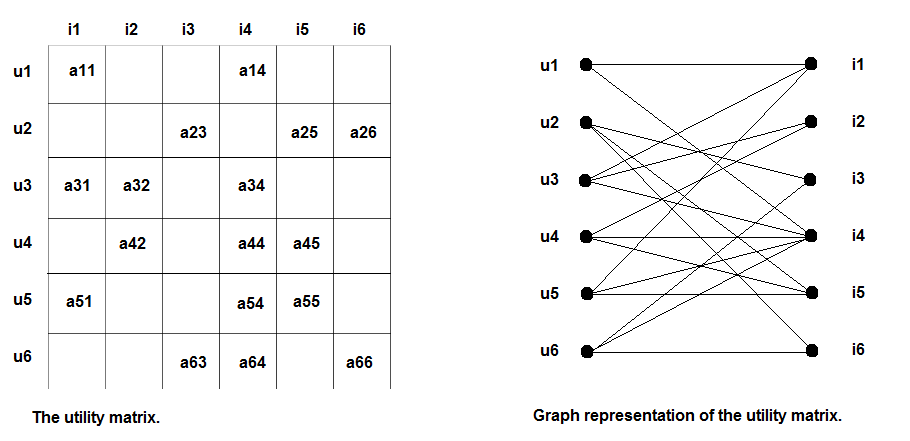
\includegraphics[width=8.3cm]{img/dualgraph}
	\caption{Transforming the utility matrix into a dual graph: two distinct sets of nodes, users and items, only share edges between nodes of different sets.}
	\label{figure:dualgraph}
\end{figure}


\subsection{Data and dimensionality reduction}\label{section:design:subsection:reduction}

Based on a visualization design by Valdis Krebs \cite{steele:2010}, a dimensionality reduction\index{dimensionality reduction} can be performed on the dual graph through \emph{row reduction}. One set of nodes is eliminated from the graph and is represented as implicit information in the edges. Figure \ref{figure:rowreduction} shows an example of this idea.

\begin{figure}
	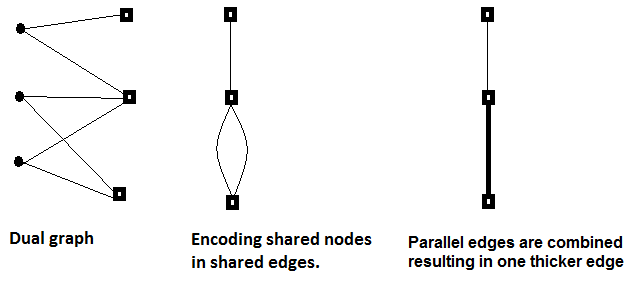
\includegraphics[width=8.3cm]{img/row_reduction}
	\caption{A row reduction operation on each pair of edges in a dual graph will result in a dimensionality reduction where one set of nodes is removed from the graph. Additional data reduction can be achieved by clustering edges into a thicker edge. Edge thickness then depends on the number of edges involved.}
	\label{figure:rowreduction}
\end{figure}

Parallel edges are retained to keep a direct link between user and edge. In the resulting visualization of the CF-based recommender, a quantification of the similarity between users can then be established by counting parallel edges between items that occur in neighbouring profiles. Figure \ref{figure:rowreduction_dualgraph} shows how the dual graph from figure \ref{figure:dualgraph} is transformed into a circular graph layout with the remaining item nodes.

\begin{figure}
	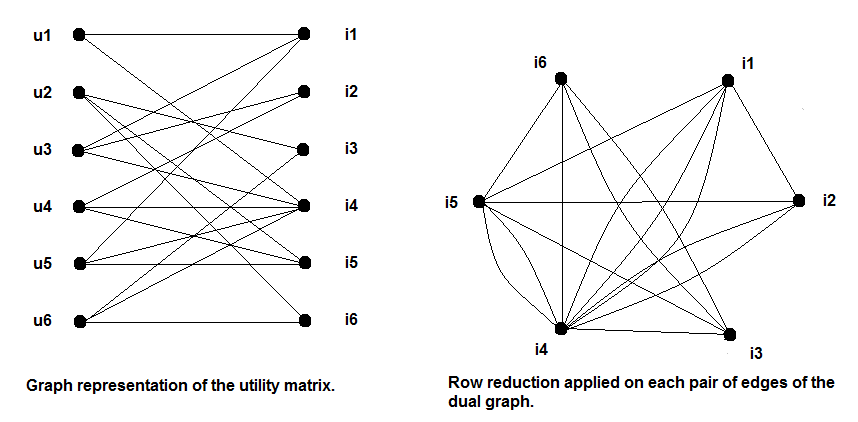
\includegraphics[width=8.3cm]{img/dualgraph_rowreduction}
	\caption{Row reduction applied on the graph in figure \ref{figure:dualgraph}.}
	\label{figure:rowreduction_dualgraph}
\end{figure}

As it is unlikely that the whole user profile can be shown in the graph while avoiding visual clutter, the active user's favourite items are used to give a representation of the active user's profile. This way the user can still directly compare him/herself with neighbouring profiles.


\subsection{Retaining contextual information}\label{section:design:subsection:contextual}

An important remark made in \cite{Klein:2006:MSS:1158821.1159015} is that data fusion algorithms can reduce information overload, but they also pose challenges to sensemaking if the human can't form an accurate mental model of the machine, to understand why and how the algorithms are doing what they are doing. Therefore, in order gain insight into the recommendation process, it is important that certain contextual information is retained. The contextual information we want to convey is two-fold:

\begin{enumerate}
	\item The strength of the links between a recommendation and the user's profile;
	\item The position of the user in his/her neighbourhood and the relation with those neighbours.
\end{enumerate}

% interaction techniques
The first type of information is contained in parallel edges between items. For the second type of information, the active user's neighbours should be included in the visualization in one way or the other. In the resulting visualization shown in figure \ref{fig:whitebox_model}, the user's top neighbours are listed next to the graph. By hovering or clicking one of the listed neighbours, the relevant parts of the graph, i.e., items owned by the neighbour and the edges between them, are highlighted.

\begin{figure}
	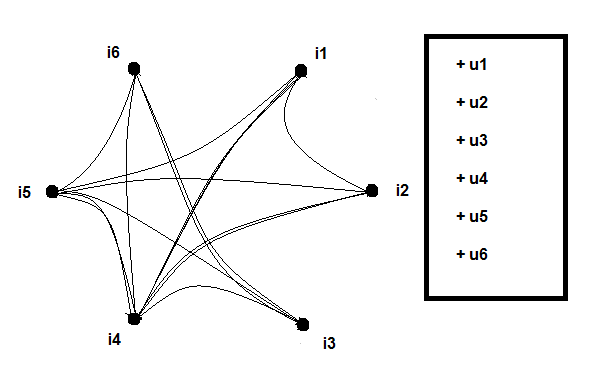
\includegraphics[width=8.3cm]{img/whitebox_model}
	\caption{The resulting visualization serving as a white box model for collaborative filtering.}
	\label{fig:whitebox_model}
\end{figure}


\section{EVALUATION}\label{section:evaluation}

A user study was conducted to evaluate the white box model presented in section \ref{section:design}. In this study the explanation system aims listed in table \ref{table:explanation:aims} are evaluated.

% objectives (cf. Tintarev's aims)

% test users, methodology
% usability (Nielsen, Duval)
% insight (North)

% procedure
\subsection{Methodology}\label{section:evaluation:subsection:methodology}

Transparency is tested by evaluating insight into the recommendation process based on North's evaluation method. We will use the think aloud protocol to obtain observational data. In particular we are looking for a user to make "domain specific inferences and hypotheses"\cite{north:2006}.

Satisfaction, efficiency, and learnability are tested through think aloud usability testing and a summative \emph{system usabiliy scale} (SUS) questionnaire. SUS is a \emph{Linkert scale} method consisting out of 10 questions, listed in figure \ref{table:sus_questions}, to investigate the subjective usability of an application\cite{brooke:1996}. Memorability is tested by asking test users that participated in previous iterations to explain the recommender rationale again at the beginning of the test.

\begin{table}
	\caption{System usability scale questions.}
	\begin{tabular}{p{15px} | p{195px} } % 210px
		\hline
		\texttt{Q1} 	&	I think that I would like to use this system frequently. \\
		\texttt{Q2}		&	I found the system unnecessarily complex. \\
		\texttt{Q3}		&	I thought the system was easy to use. \\
		\texttt{Q4} 	&	I think that I would need the support of a technical person to be able to use this system. \\
		\texttt{Q5}		&	I found the various functions in this system were well integrated. \\
		\texttt{Q6}		&	I thought there was too much inconsistency in this system. \\
		\texttt{Q7} 	&	I would imagine that most people would learn to use this system very quickly.  \\
		\texttt{Q8}		&	I found the system very cumbersome to use. \\
		\texttt{Q9}		& I felt very confident using the system. \\
		\texttt{Q10}	& I needed to learn a lot of things before I could get going with this system. \\
		\hline
	\end{tabular}
	\label{table:sus_questions}
\end{table}

Trust, persuasiveness, and effectiveness are evaluated through direct feedback from the test subjects.

\subsection{Participants}\label{section:evaluation:subsection:setup}
% conceptual model evaluated by 15 test users through a series of iterations
% increase domain relevance: visualization in the Last.fm page + Last.fm users

Test users were selected from the campus and among acquaintances and were between 21 and 26 years of age. For all of the iterations combined, a total of 15 users participated in the user study of whom 12 were male and 3 were female. All users had an interest in music and listened actively to music at least once a day. Although they had a notion of what a recommender system was, none of them knew how recommendation algorithms worked.

Nielsen \cite{nielsen:2012:nngroup:diminishing_returns} proposes to make iterations short by limiting the number of test users. He argues that five test users per iteration are enough to find most of the usability issues. By iterating and addressing surfaced usability issues between each iteration, after a couple of iterations all usability problems will have been resolved.

As a result, the test users were spread among four different iterations. Some of the users participated in multiple tests to provide direct feedback on changes made between the iterations. The distribution of users can be seen in table \ref{table:evaluation:users}.

\begin{table}
	\caption{The distribution of test users used in the evaluations for each iteration.}
	\begin{tabular}{l | l l l l }
		\hline
															& \multicolumn{4}{c}{\textbf{Iteration}} \\
															\cline{2-5}
															& $1$ & $2$ & $3$ & $4$ \\
		\hline
		Number of users						&	5 	&	5		&	5		&	10	\\
		From previous iterations	&	-  	&	2 	&	3		&	5	\\
		\hline
	\end{tabular}
	\label{table:evaluation:users}
\end{table}




\subsection{Prototyping}\label{section:evaluation:subsection:prototyping}

Over the four iterations the application was incrementally improved. Table \ref{table:iteration:aims} gives an overview of which aims were evaluated for the prototype in each iteration.

\begin{table}
	\caption{The explanation aims that were evaluated in each iteration.}
	\begin{tabular}{l | l l l l }
		\hline
		\textbf{Aim} 							& \multicolumn{4}{c}{\textbf{Iteration}} \\
															\cline{2-5}
															& $1$ & $2$ & $3$ & $4$ \\
		\hline
		Tra. Sat., Efc., Learn.		&	x 	&	x		&	x		&	x	\\
		Mem.											&	  	&	x		&	x		&	x	\\
		Trust, Efk., Pers.				&	  	&	 		&	 		&	x	\\
		\hline
	\end{tabular}
	\label{table:iteration:aims}
\end{table}

%Efficiency is measured by comparing the time it took to arrive at insight into the recommendation rationale for different users, as well as using results.

The first prototype, shown in figure \ref{figure:paper_prototype}, was made out of paper. \emph{Paper prototypes} are relatively easy and cheap to make. Evaluation of this kind of prototype allows to detect usability problems at an early stage in the development process at a low cost. This avoids having to fix these usability problems in an actual implementation, which is much more expensive\cite{snyder:2003}.

The second prototype, displayed in figure \ref{figure:prototype_soundsuggest1}, is an implementation of the visualization using the \texttt{D3} \emph{JavaScript} library. This version uses the same static data as in the paper prototype. In addition to the aims listed in table \ref{table:iteration:aims}, the success of the conversion from paper to digital prototype is evaluated as well.

The third prototype uses the visualization in a Chrome browser extension that is injected into the \emph{Last.fm} recommendations page\footnote{\url{http://www.last.fm/home/recs}}. The visualization uses live data from the logged in user. This, in combination with the context of the Last.fm website, increases the domain relevance for insight evaluation. The main objective of the user study for this prototype was to find usability issues before moving on to a test with more users.

In the final prototype all of the other aims were evaluated, apart from scrutability, as this was not supported by Last.fm's API\footnote{\url{http://www.last.fm/api}}. An example of the visualization is shown in figure \ref{figure:prototype_soundsuggest3}.



\subsection{Results}\label{section:evaluation:subsection:results}

% results for each aim
% 	- usability (satisfaction)
%		- insight (transparency)
%		- other

\subsubsection{Transparency}

All test users were able to derive the recommendation rationale from the visualization. However, there were some differences in the speed of the insight gaining process.

The test was designed to better distinguish between the steps of the insight gaining process. To simulate the first step, \emph{provide overview}, users were asked to form an initial mental model before interacting with the visualization. For all iterations most users saw the edges as content-based relationships, e.g. artists are connected based on genre. Only two users managed to get the visualization rationale right the first time. Based on the visualization they were able to describe the recommendation rationale.

\emph{Adjust}, \emph{detect pattern}, and \emph{match mental model} were simulated in the next part of the test by allowing interaction with the visualization. Users could now dig deeper into the data model, gaining understanding about relationships among its elements. It should be noted that over the iterations, changes in the amount of data displayed, as well as changes in the graph's layout had an influence on the insight gaining speed.

In the first iteration, see figure \ref{figure:paper_prototype}, parallel edges were clearly visible, whereas in the other iterations, see for example figure \ref{figure:prototype_soundsuggest1}, Holten's edge-bundling algorithm made parallel edges overlap. Test users indicated that this made it harder to see the link between the number of edges between an artist, and the number of highlighted neighbours. This was also supported by observational data, as this kind of stories did no longer occur in think aloud tests, unless insight into visualization's rationale had already been gained via another way.

As the number of data elements displayed increased, comparing prototypes in figures \ref{figure:prototype_soundsuggest1} and \ref{figure:prototype_soundsuggest3}, it became harder to gain insight, as the total amount of edges made it harder to distinguish between them. This is probably to be expected, as small graphs are easier to analyze\cite{herman:2000}.

Usually the visualization rationale learned when the user saw that a user profile corresponded to set of interconnected nodes. By comparing overlaps between artist node sets and the highlighted active profile, they understood how neighbouring profiles were interrelated, and how recommendations were computed.


\subsubsection{Satisfaction, efficiency, learnability and memorability}

To get an idea of the perceived usability, the SUS questionnaire results are used. These changed over the iterations: new users were introduced and the design changed over time. Also, when comparing the first iteration with the others, the interaction with a paper prototype is still rather different than working with a digital version. The results are shown in figure \ref{fig:iterations_sus_scores_boxplots}.

\begin{figure}
	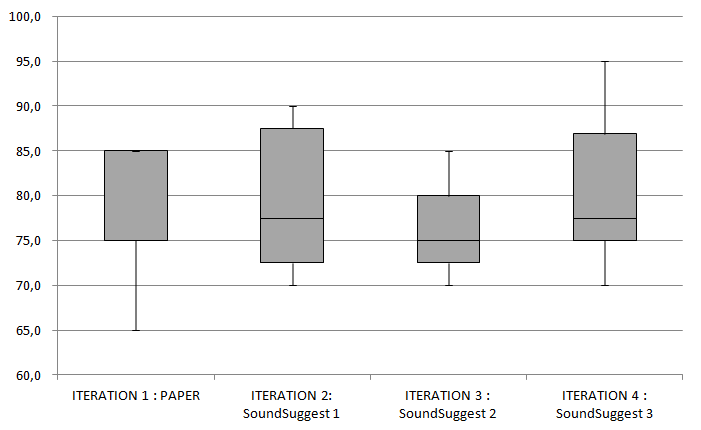
\includegraphics[width=8.3cm]{img/iterations_sus_scores_boxplots}
	\caption{The SUS results for each iteration, visualized as box plots.}
	\label{fig:iterations_sus_scores_boxplots}
\end{figure}


Figures \ref{fig:iterations_sus_scores_it1_boxplots} to \ref{fig:iterations_sus_scores_it4_boxplots} show the distribution of answers for each iteration. The questions with the lowest scores overall were the first question and the seventh question.

% This may on the other hand, have decreased domain relevance ...
Low scores on \texttt{Q1} may point to low satisfaction, but at the same time there were very positive remarks as well. Another explanation might be that low scores correspond to users that simply don't use Last.fm frequently. Based on the results for \texttt{Q3}, the majority of test users indicated that they thought the application was easy to use.

Although there were no negative votes for \texttt{Q7}, a lot of users were not convinced that using the application was easy to learn. Although the results for \texttt{Q10} suggest otherwise based on iteration 2 and 4, this question might be more prone to possible bias introduced during the test, which is perhaps confirmed by results for \texttt{Q4} in iteration 1 and 3.

Even though the application did not stay exactly the same over the iterations, test users that took part in two or more user tests were able to apply their experience from the previous test to the new test. Recalling the recommender rationale sometimes required some familiarization with the application again.



\subsubsection{Persuasion, effectiveness, and trust}

% recommender bias --> bad recommendations --> lower trust
% recommendations that people know and like --> increase trust
% known : possibly forgotten about
% recommendations not known --> good recommendations --> increase trust (more)
% recommendations not known --> bad recommendations --> lower trust (more)
% new : possibly more interesting

In terms of trust, four scenarios were investigated: effective/bad, known/new recommendations.

It turns out the Last.fm recommender has some bias towards certain clusters of artists. Artists from a smaller music scene tend to be affected by regional effects. For example according to Last.fm, a similar artist to \emph{De Kreuners}, a Belgian rock band, is \emph{Samson \& Gert}, a performer of music targeted to children. Another example is that bands that have certain musicians in common often are considered similar, even though their music styles are not. Usually test users already knew about these artists and indicated that this decreased their trust in the recommender system.

Similarly, bad recommendations that were new to the user also decreased trust in the recommendations.

Not all test users received this kind of biased recommendations and effective recommendations would increase the user's trust in the recommender system. Good new recommendations would increase their trust in the system more than artists they already knew about.

In some cases the explanation system helped to identify bad recommendations, as the active user's top neighbours would not have these items in their profile.

As users gained insight in the visualization and the recommender system behind it, the user's trust in the system increased as well. Persuasion was harder to measure. Typically test users would look for artist nodes where a lot of edges originated from, or users with a high similarity score.

Although the explanation system was not always as effective in helping to find good recommendations, it provided an additional means for the user to establish his/her own approach for finding recommendations. For example a user would look at neighbours for artist suggestions, rather than just the artist recommendations by Last.fm.


\section{CONCLUSION AND FUTURE WORK}\label{section:conclusion}

% usability
% Tintarev criteria
% insight?

% learnability: disspointing
% insight: is possible
% In conclusion there might still be some work left to make the application more accessible to casual users.

% modifying links between items to adjust recommender 'memory': if people create their own links within a profile without having everything in their profile linked together --> possibly better recommendations

% neighbour listening history for a recommendation

This paper has described a visual explanation system collaborative recommendation. The design was evaluated through user studies, first as a paper prototype which was later implemented as a Chrome Extension for the Last.fm website to explain its music recommendations. We used aims proposed by Tintarev and Masthoff, with additional usability metrics listed by Nielsen to evaluate these prototypes.

Results indicate that our design can be effective in explaining the rationale of collaborative recommendations. However, the learnability of the system still has some room for improvement. An overall SUS score in the final iteration of $80.5$ suggests that the usability of the system is good, as perceived by users. Finally, the explanation system can help increase trust in the recommender system and may provide a starting point for further data exploration.

To improve the application, issues such as data density, slow data loads should be addressed further. It would also be interesting to see how the explanation system would perform for another collaborative recommender system.

%To improve the evaluation methods


\bibliographystyle{abbrv}
\bibliography{bib/references}



\begin{appendices}
  
	% BEGIN FIGURE : paper prototype
	\begin{figure*}
		\centering
		\begin{subfigure}[t]{0.3\textwidth}
						\centering
						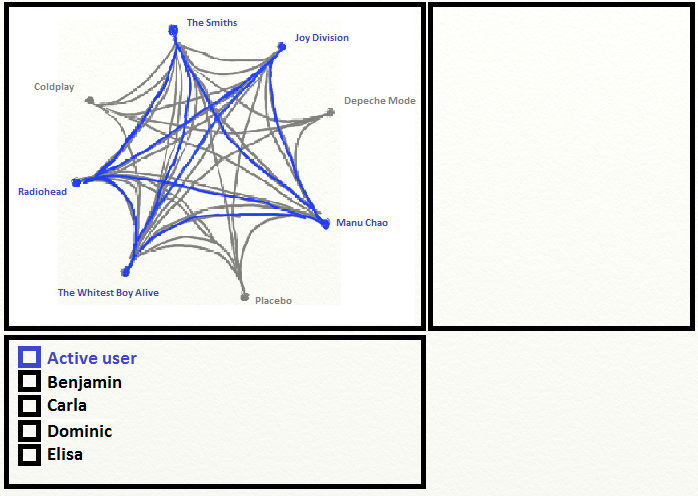
\includegraphics[width=\textwidth]{img/paper_prototype_default}
						\caption{The default visualization with the active user's items highlighted.}
						\label{figure:paper_prototype_default}
		\end{subfigure}%
		~
		\begin{subfigure}[t]{0.3\textwidth}
						\centering
						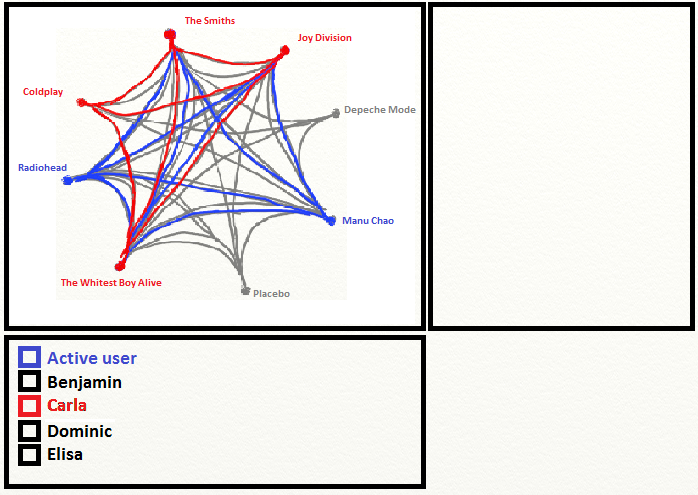
\includegraphics[width=\textwidth]{img/paper_prototype_user_click}
						\caption{Clicking a user list element.}
						\label{figure:paper_prototype_user_click}
		\end{subfigure}
		~
		\begin{subfigure}[t]{0.3\textwidth}
						\centering
						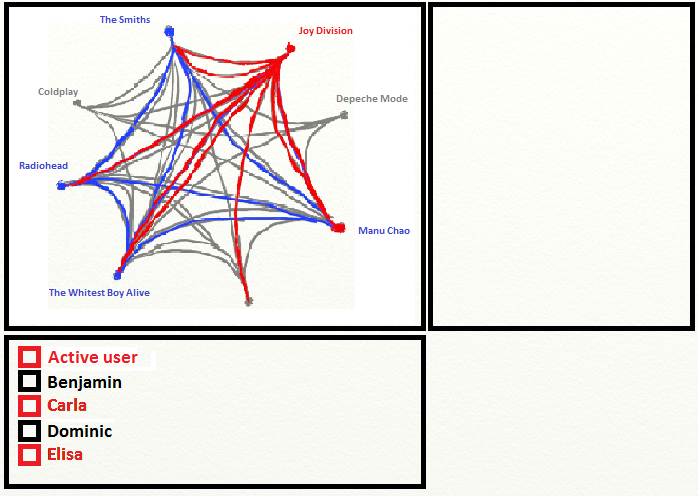
\includegraphics[width=\textwidth]{img/paper_prototype_item_click}
						\caption{Clicking an item node.}
						\label{figure:paper_prototype_item_click}
		\end{subfigure}
		\caption{A selection of the screens used in the user study with paper prototype.}%
		\label{figure:paper_prototype}%
	\end{figure*}

	% ITERATION 2
	\begin{figure*}
		\centering
		\begin{subfigure}[t]{0.3\textwidth} % t for top alignment, b for bottom
						\centering
						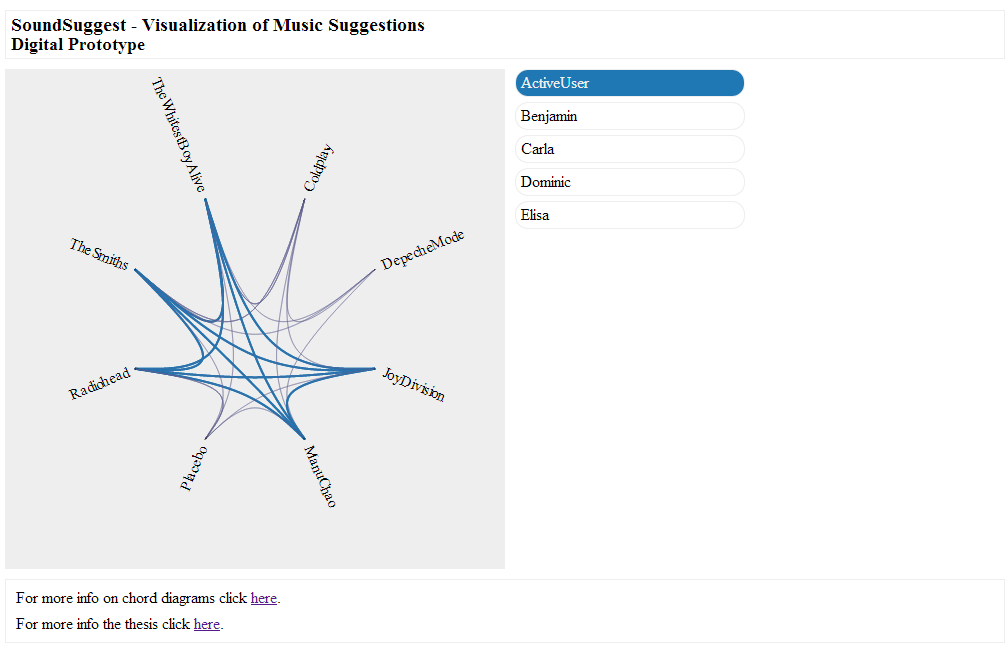
\includegraphics[width=\textwidth]{img/prototype_soundsuggest1_default}
						\caption{The default visualization with the active user's items highlighted.}
						\label{figure:prototype_soundsuggest1_default}
		\end{subfigure}%
		~
		\begin{subfigure}[t]{0.3\textwidth}
						\centering
						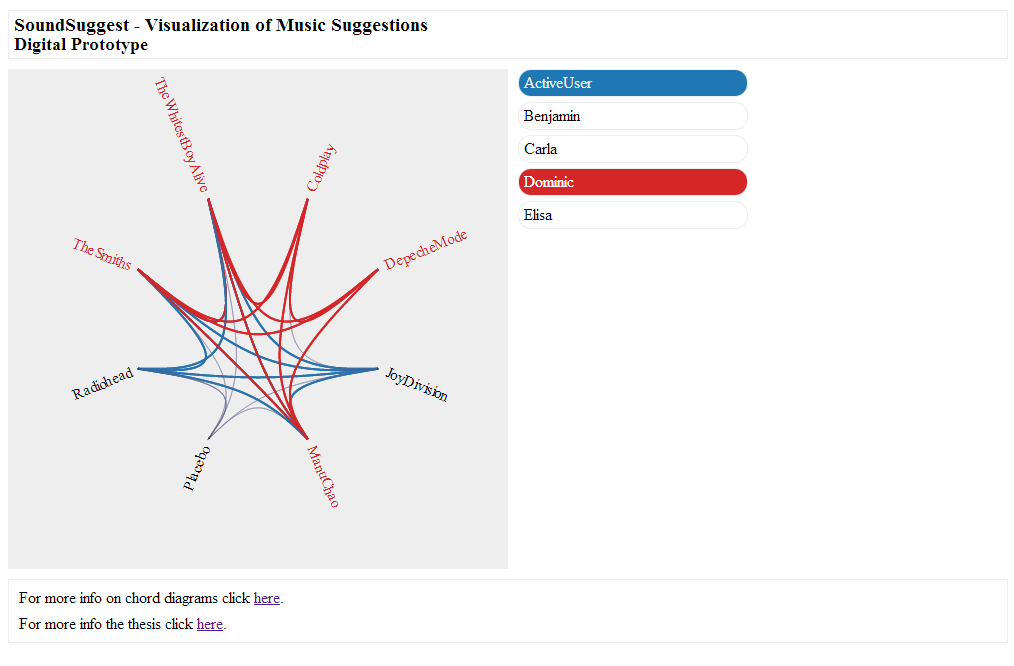
\includegraphics[width=\textwidth]{img/prototype_soundsuggest1_user_click}
						\caption{Clicking a user list element.}
						\label{figure:prototype_soundsuggest1_user_click}
		\end{subfigure}
		~
		\begin{subfigure}[t]{0.3\textwidth}
						\centering
						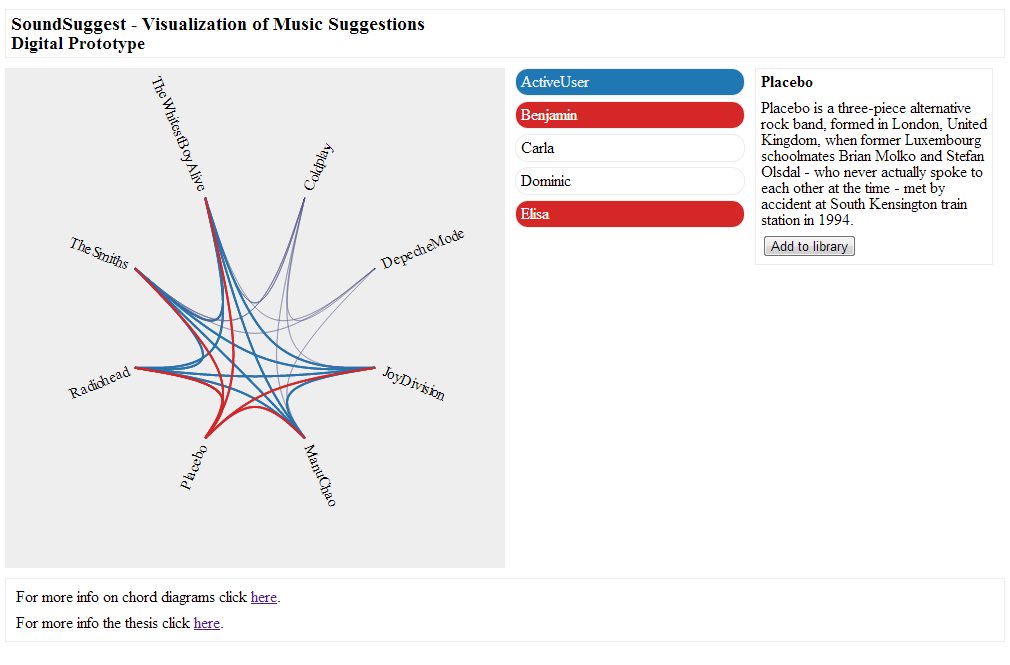
\includegraphics[width=\textwidth]{img/prototype_soundsuggest1_item_click}
						\caption{Clicking an item node.}
						\label{figure:prototype_soundsuggest1_item_click}
		\end{subfigure}
		\caption{A selection of the screens used in the user study with the first digital prototype.}%
		\label{figure:prototype_soundsuggest1}%
	\end{figure*}

	% ITERATION 3
	\begin{figure*}
		\centering
		\begin{subfigure}[t]{0.3\textwidth}
						\centering
						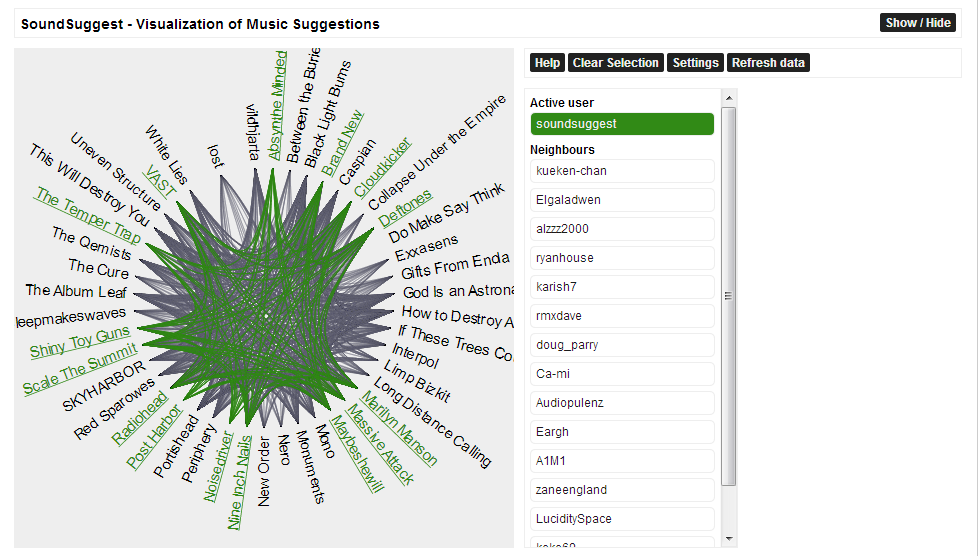
\includegraphics[width=\textwidth]{img/prototype_soundsuggest3_default}
						\caption{The default visualization with the active user's items highlighted.}
						\label{figure:prototype_soundsuggest3_default}
		\end{subfigure}%
		~
		\begin{subfigure}[t]{0.3\textwidth}
						\centering
						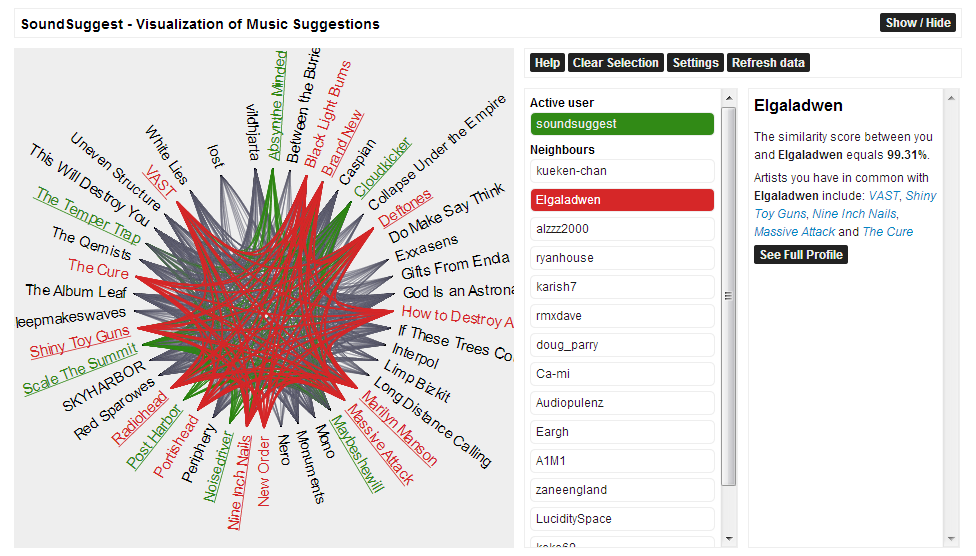
\includegraphics[width=\textwidth]{img/prototype_soundsuggest3_user_click}
						\caption{Clicking a user list element.}
						\label{figure:prototype_soundsuggest3_user_click}
		\end{subfigure}
		~
		\begin{subfigure}[t]{0.3\textwidth}
						\centering
						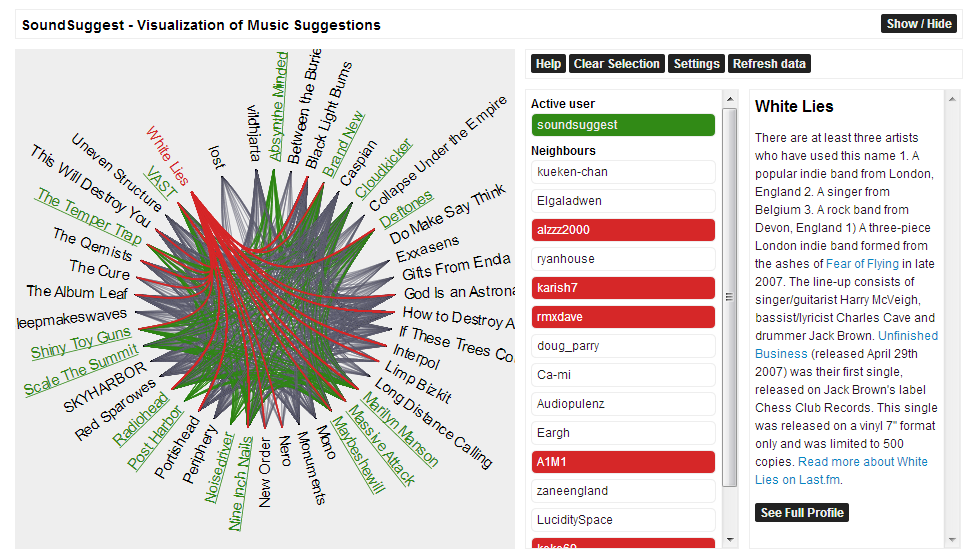
\includegraphics[width=\textwidth]{img/prototype_soundsuggest3_item_click}
						\caption{Clicking an item node.}
						\label{figure:prototype_soundsuggest3_item_click}
		\end{subfigure}
		\caption{A selection of the screens used in the user study with the third digital prototype.}%
		\label{figure:prototype_soundsuggest3}%
	\end{figure*}
	
	\begin{figure}
		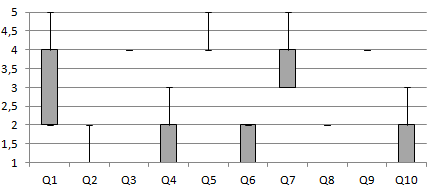
\includegraphics[width=8.3cm]{img/iterations_sus_scores_it1_boxplots}
		\caption{The SUS results for each question for iteration 1.}
		\label{fig:iterations_sus_scores_it1_boxplots}
	\end{figure}

	\begin{figure}
		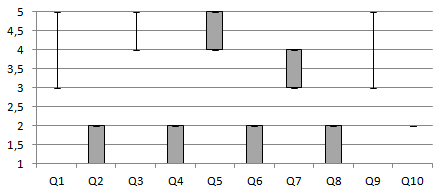
\includegraphics[width=8.3cm]{img/iterations_sus_scores_it2_boxplots}
		\caption{The SUS results for each question for iteration 2.}
		\label{fig:iterations_sus_scores_it2_boxplots}
	\end{figure}

	\begin{figure}
		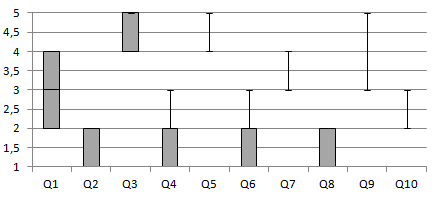
\includegraphics[width=8.3cm]{img/iterations_sus_scores_it3_boxplots}
		\caption{The SUS results for each question for iteration 3.}
		\label{fig:iterations_sus_scores_it3_boxplots}
	\end{figure}

	\begin{figure}
		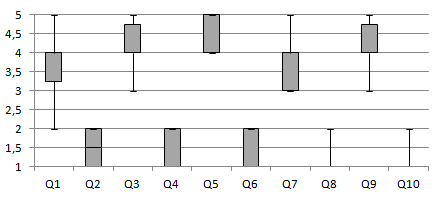
\includegraphics[width=8.3cm]{img/iterations_sus_scores_it4_boxplots}
		\caption{The SUS results for each question for iteration 4.}
		\label{fig:iterations_sus_scores_it4_boxplots}
	\end{figure}
	
\end{appendices}

\end{document}
